% latexmk -pdflatex='xelatex %O %S' -pvc -pdf slides.tex
\documentclass{beamer}

\beamertemplatenavigationsymbolsempty

% für xelatex:
\usepackage{xltxtra}
\usepackage{unicode-math}

% literatur
\usepackage[backend=biber,style=alphabetic]{biblatex}

\addbibresource{../util/literature.bib}

\usepackage{../util/zariski}

\usepackage{csquotes}
\usepackage{hyperref}
\usepackage{tikz}
\usetikzlibrary{cd,arrows,shapes,calc,through,backgrounds,matrix,trees,decorations.pathmorphing,positioning,automata}
\usepackage{graphicx}
\usepackage{color}

\usepackage{mathpartir}
\newcommand{\yields}{\vdash}
\newcommand{\cbar}{\, | \,}


% für tabellen
\usepackage{booktabs}

\title[ConCoh]
{\v{C}ech Cohomology in Homotopy Type Theory}
\author[Author, Anders] 
{Ingo Blechschmidt, Felix Cherubini, David Wärn}

\begin{document}

\date{}
\begin{frame}
  \titlepage
\end{frame}

\begin{frame}
  Part of the synthetic \href{https://github.com/felixwellen/synthetic-zariski/blob/main/README.md}{algebraic geometry project}:
  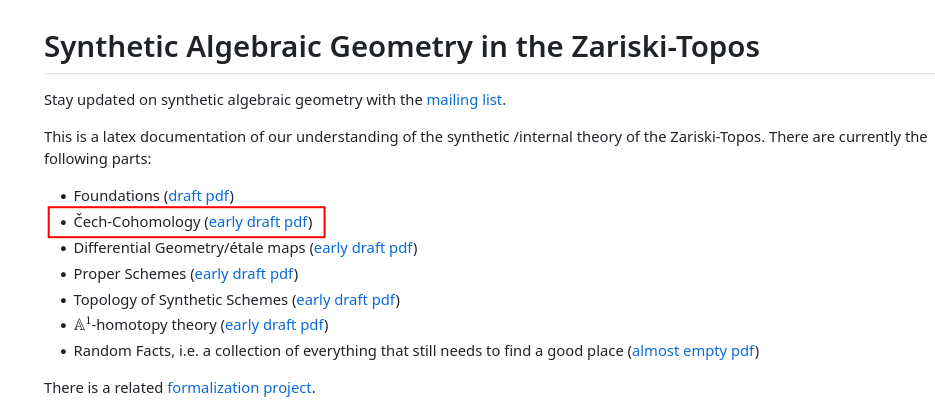
\includegraphics[width=9cm]{project-cech.png}
\end{frame}

\begin{frame}
  \vspace{1cm}
  \begin{center}
    \begin{tikzpicture} 
      [ 
      node distance=.8cm, 
      circled/.style={draw, ellipse, ultra thick, fill=blue!12},
      edge from parent/.style={very thick,draw=black,-latex},
      plaintext/.style={}
      ]

      \tikzstyle{level 1}=[sibling angle=81,level distance=4cm]

      \node[circled] (hott) {HoTT+Axioms} [counterclockwise from=207]
      child { 
        node[circled] (grp) {$\infty$-Groupoids} 
        edge from parent [-latex] node (grp) 
        {
          \begin{tikzpicture}[scale=0.8, rotate=25]
            \draw[-, red, ultra thick] (0,0) to (1,1);
            \draw[-, red, ultra thick] (1,0) to (0,1);
          \end{tikzpicture}
        } 
      }
      child { node[matrix, circled, inner sep=0pt] (smgrp) 
        {
          \node[circled, minimum height=0.7cm, minimum width=3cm] (mfd) {Schemes};
          \node[below of=mfd, text width=3cm,
          node distance=0.9cm] 
          {``Constructive Zariski-sheaves''}; \\
        }
      }
      ;
    \end{tikzpicture}
  \end{center}
  \vspace{1cm}
  {\footnotesize * Schemes = quasi-compact, quasi-separated schemes of finite type}
\end{frame}

\begin{frame}
  \frametitle{Reminder: The 3 Axioms}
  \textbf{Axiom:} We have a local, commutative ring $R$. \\

  \vspace{0.25cm}
  For a finitely presented $R$-algebra $A$, define:
  \[ \Spec(A):\equiv \Hom_{R\text{-algebra}}(A,R)\]

  \textbf{Axiom (synthetic quasi-coherence (SQC)):} \\
  For any finitely presented $R$-algebra $A$, the map
  \[ a\mapsto (\varphi\mapsto \varphi(a)):A \xrightarrow{\sim} R^{\Spec(A)} \]
  is an equivalence.

  \textbf{Axiom (Zariski-local choice):}\\
  For every surjective $\pi$, there merely exist local sections $s_i$
  \[ \begin{tikzcd}[ampersand replacement=\&, column sep=small]
    \& E \ar[d, two heads, "\pi"] \\
    D(f_i) \ar[r, hook] \ar[ur, bend left, dashed, "s_i"] \& \Spec(A)
  \end{tikzcd} \]
  with $f_1, \dots, f_n : A$ coprime.
\end{frame}

\begin{frame}
  \vspace{0.25cm}
  For $A : X \to \mathrm{Ab}$, define \emph{cohomology} as:
  \[ H^n(X, A) :\equiv \Big\| \prod_{x:X}K(A_x,n) \Big\|_{\mathrm{set}} \]
  
  \pause
  Good because:
  \begin{itemize}
  \item $\prod$-type.
  \item Homotopy group: $H^n(X,A)=\pi_{k}(\prod_{x:X}K(A,n+k))$.
  \item $\|\_\|_{\mathrm{set}}$ is a modality.
  \end{itemize}

  \pause
  Non-trivial for $X:\mathrm{Set}$ because:

  $X=$ Pushout of sets $U\leftarrow Y\to V$, \\
  Then a ``cohomology class'' $X\to K(A,1)$ is given by:
  \begin{itemize}
  \item Maps $f:U\to K(A,1)$, $g:V\to K(A,1)$.
  \item And $h:(x:Y)\to f(x)=g(x)$, which is essentially a map $Y\to A$,
    if $U$ and $V$ don't have higher cohomology...
  \end{itemize}
\end{frame}


\ignore{
    \item $H^n(X,M)=0$ if $n>0$, $X$ is affine and $M:X\to \Mod{R}_{\mathrm{wqc}}$.
  \item $H^n(X,M)$ coincides with \v{C}ech-Cohomology (for \emph{separated} schemes).
  \item By work of Blechschmidt and Wärn: A scheme $X$ is affine if and only if
      \[ H^n(X, M) = 0 \]
      for all $M : X \to R\text{-}\mathrm{Mod}_{\mathrm{wqc}}$ and $n > 0$.

}

\begin{frame}
  \frametitle{Mayer-Vietoris Sequence}
  $X=U\cup V$ (or some other pushout). Then the following is exact:
  \begin{center}
    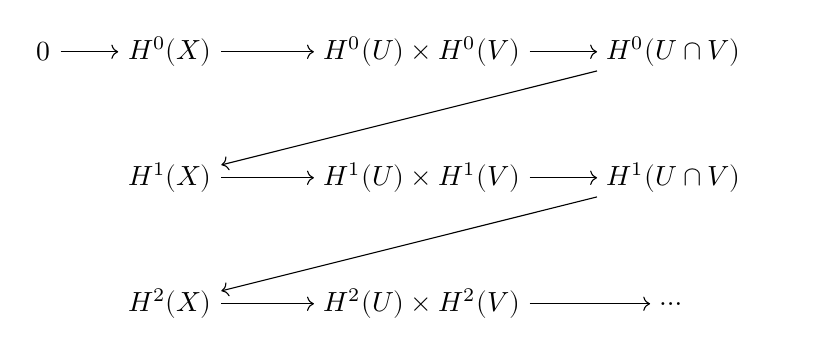
\begin{tikzpicture}[node distance=1.6cm, auto]
      \node (zero) {$0$};
      
      \node[right of=zero] (H0X)               {$H^0(X)$};
      \node[below of=H0X] (H1X) {$H^1(X)$};
      \node[below of=H1X] (H2X) {$H^2(X)$};
      \node[right of=H0X] (Space1) {$ $}; % ugly hack
      
      \node[right of=Space1]   (H0UxV) {$H^0(U)\times H^0(V)$};
      \node[below of=H0UxV] (H1UxV) {$H^1(U)\times H^1(V)$};
      \node[below of=H1UxV] (H2UxV) {$H^2(U)\times H^2(V)$};
      \node[right of=H0UxV] (Space2) {$ $};
      
      \node[right of=Space2] (H0UV) {$H^0(U\cap V)$};
      \node[below of=H0UV]  (H1UV) {$H^1(U\cap V)$};
      \node[below of=H1UV]  (H2UV) {$\dots$};
      \node[right of=H2UV] (Space3) {$ $};

      \draw[->] (zero) to (H0X);
      
      \draw[->] (H0X) to (H0UxV);
      \draw[->] (H1X) to (H1UxV);
      \draw[->] (H2X) to (H2UxV);
      
      \draw[->] (H0UxV) to (H0UV);
      \draw[->] (H1UxV) to (H1UV);
      \draw[->] (H2UxV) to (H2UV);

      \draw[->] (H0UV) to (H1X);
      \draw[->] (H1UV) to (H2X);
      
    \end{tikzpicture}
  \end{center}
\end{frame}

\begin{frame}
  \frametitle{Examples: Cohomology of Pushouts}
  \begin{minipage}{.5\textwidth}
    \begin{tikzpicture}[node distance=1.6cm, auto]
      \node (Ax) {$\A^\times$};
      \node[right of=Ax] (A1r) {$\A^1$};
      \node[below of=Ax] (A1l) {$\A^1$};
      \node[right of=A1l] (A1dp) {$\A^1_{..}$};
      
      \draw[->] (Ax) to (A1r);
      \draw[->] (Ax) to (A1l);
      \draw[->] (A1l) to (A1dp);
      \draw[->] (A1r) to (A1dp);
    \end{tikzpicture}
  \end{minipage}
  \begin{minipage}{.4\textwidth}
    \[
      \A^1_{..}
    \]
    \begin{tikzpicture}[node distance=2cm]
      \node (left) {$ $};
      \node[right of=left] (middle) {$\circ$};
      \node[right of=middle] (right) {$ $};

      \draw[shorten >=2pt] (left) to ([yshift = 0.5pt] middle.center);
      \draw[shorten <=2pt] ([yshift = 0.5pt] middle.center) to (right);
    \end{tikzpicture}
  \end{minipage}
  \pause
  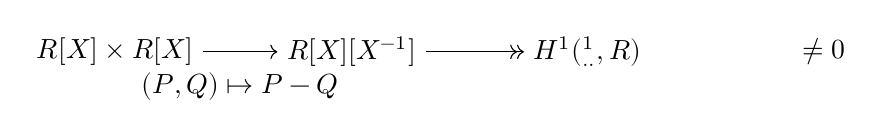
\begin{tikzpicture}[node distance=3cm]
    \node (RR) {$R[X]\times R[X]$};
    \node[right of=RR] (RI) {$R[X][X^{-1}]$};
    \node[right of=RI] (H1) {$H^1(\A^1_{..},R)$};
    \node[right of=H1] {$\neq 0$};

    \draw[->] (RR) to node[below,yshift=-4pt] {$(P,Q)\mapsto P-Q$} (RI);
    \draw[->>] (RI) to (H1);
  \end{tikzpicture}

  \vspace{.5cm}
  \pause
  \begin{minipage}{.5\linewidth}
    \begin{tikzpicture}[node distance=1.6cm, auto]
      \node (Ax) {$\A^\times$};
      \node[right of=Ax] (A1r) {$\A^1$};
      \node[below of=Ax] (A1l) {$\A^1$};
      \node[right of=A1l] (A1dp) {$\bP^1$};
      
      \draw[->] (Ax) to (A1r);
      \draw[->] (Ax) to node[swap] {$\frac{1}{x}$} (A1l);
      \draw[->] (A1l) to (A1dp);
      \draw[->] (A1r) to (A1dp);
    \end{tikzpicture}
  \end{minipage}
  \begin{minipage}{.4\linewidth}
    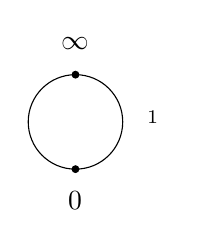
\begin{tikzpicture}
      \draw (0,0) circle [radius=0.6cm];
      \fill (0,0.6cm) circle [radius=0.05cm];
      \fill (0,-0.6cm) circle [radius=0.05cm];
      
      \node (M) at (0,0) {$ $};
      \node[above of=M] {$\infty$};
      \node[below of=M] {$0$};
      \node[right of=M] {$ \bP^1$};
    \end{tikzpicture}
  \end{minipage}
  \pause
  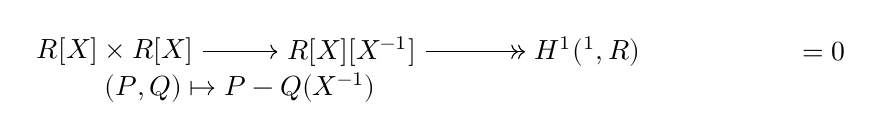
\begin{tikzpicture}[node distance=3cm]
    \node (RR) {$R[X]\times R[X]$};
    \node[right of=RR] (RI) {$R[X][X^{-1}]$};
    \node[right of=RI] (H1) {$H^1(\bP^1,R)$};
    \node[right of=H1] {$=0$};

    \draw[->] (RR) to node[below,yshift=-4pt] {$(P,Q)\mapsto P-Q(X^{-1})$} (RI);
    \draw[->>] (RI) to (H1);
  \end{tikzpicture}

\end{frame}

\begin{frame}
  \frametitle{Vanishing on Affine Schemes}
  \begin{theorem}
    Let $X=\Spec A$, $n>0$ and $M:X\to \Mod{R}_{\mathrm{wqc}}$, then
    \[
      H^n(X,M)=0
      \rlap{.}
    \]
  \end{theorem}
  \pause
  \begin{proof}
    Uses: Homotopy theory, algebra, Zariski-local choice and properties of wqc-modules.
  \end{proof}
\end{frame}

\begin{frame}
  \frametitle{Applying Cohomology}
  To (merely) construct functions, one can use exactness of:
  \[
    0\to \prod_{x:X}M_x\to \prod_{x:X}N_x\to \prod_{x:X}K_x\to H^1(X,M)
  \]
  (which holds if $0\to M_x\to N_x\to K_x\to 0$ is exact for all $x:X$)

  \vspace{1.3cm}
  \pause
  To show a scheme is affine!

  This holds if for all $I:X\to \Mod{R}_{\mathrm{wqc}}$ such that $I_x$ is an ideal in $R$ for all $x:X$,
  we have $H^1(X,I)=0$, by a recent theorem of Ingo Blechschmidt and David Wärn.
\end{frame}

\begin{frame}
  \frametitle{\v{C}ech-Cohomology}
  Generalization of Mayer-Vietoris for spaces $X=\bigcup_{i=1}^nU_i$, where $U_i$ and all their $k$-ary intersections have trivial higher cohomology.
  
  \pause
  By Vanishing, separated schemes with their open affine cover, are an example.
  
  \pause
  Two proofs:
  \begin{itemize}
  \item By universal property, that both \v{C}ech and Eilenberg-MacLane cohomology have.
  \item Roughly, by pointwise turning the colimit $U_1(x)\vee\dots\vee U_n(x)$ into a limit.
  \end{itemize}
\end{frame}

\begin{frame}
  \centering
  Thank you!
\end{frame}

\end{document}
